\documentclass[8pt,landscape]{article}

% PACKAGES
\usepackage[letterpaper, margin=0.1in]{geometry}
\usepackage{amsmath, amssymb, geometry}
\usepackage{multicol}
\usepackage{setspace}
\usepackage{sectsty}
\usepackage{verbatim}
\usepackage{graphicx}
\usepackage{xcolor}
\usepackage{listings}
\usepackage{enumitem}
\usepackage{booktabs} % For better tables if needed

% Define a custom color for code highlighting and environment
\definecolor{myred}{RGB}{204, 0, 0} % A strong red
\definecolor{mygray}{RGB}{240, 240, 240} % Light gray for background
\setlist[itemize]{
    noitemsep,  % Removes vertical space between list items
    topsep=0pt,  % Removes space before the list
    partopsep=0pt, % Removes extra space when a list begins mid-paragraph
    parsep=0pt, % Removes space between paragraphs within an item
    leftmargin=*, % Sets the left margin to the minimum necessary
    labelsep=0.5em, % You can slightly adjust the space between the bullet and the text
}
% LISTINGS SETUP for R and Python
\lstset{
  basicstyle=\ttfamily\scriptsize\color{black},
  backgroundcolor=\color{mygray},
  frame=single,
  frameround=tttt,
  framesep=0pt,        % no padding between code and frame
  rulecolor=\color{black!20},
  rulesep=0pt,         % no space between rules
  breaklines=true,
  columns=fullflexible,
  showstringspaces=false,
  commentstyle=\color{gray},
  keywordstyle=\color{blue!80!black},
  stringstyle=\color{myred},
  breakatwhitespace=true,
  xleftmargin=0pt,     % no left margin
  xrightmargin=0pt,    % no right margin
  aboveskip=0pt,       % no space above listing
  belowskip=0pt,       % no space below listing
  abovecaptionskip=0pt,
  belowcaptionskip=0pt,
  framexleftmargin=0pt,
  framexrightmargin=0pt,
  framextopmargin=0pt,
  framexbottommargin=0pt
}

% FORMATTING
\setstretch{0.9} % Reduce line spacing
\setlength{\parindent}{0pt}
\setlength{\parskip}{0pt}

% Reduce section spacing and change color
\makeatletter
\renewcommand{\section}{\@startsection{section}{2}{0pt}%
    {0.1ex}% space before section
    {0.1ex}% space after section
    {\fontsize{8}{9}\bfseries\color{red}}} % section font: 8pt
\makeatother

% Reduce subsection spacing and make subsections blue
\makeatletter
\renewcommand{\subsection}{\@startsection{subsection}{2}{0pt}%
    {0.1ex}% space before subsection
    {0.1ex}% space after subsection
    {\fontsize{8}{9}\bfseries\color{blue}}} % Subsection font: 8pt
\makeatother

% Custom command for red-highlighted code/commands (for in-line use)
\newcommand{\code}[1]{\textcolor{myred}{\texttt{#1}}}

% Custom small text wrapper - ensuring 8pt for body text
\newcommand{\smalltext}[1]{
  {\fontsize{8}{9}\selectfont\sloppy #1\par}
}

% DOCUMENT START
\begin{document}
\fontsize{8}{9}\selectfont % Set the base font size to 8pt and line skip to 9pt for the entire document
\pagestyle{empty}
\begin{multicols}{3}

\section{Probabilistic Forecasting}
\smalltext{
Probabilistic forecasting moves beyond point forecasts (averages) to estimate uncertainty, predicting extremes like the 90th quantile or future volatility. Main sources of uncertainty include random error, model parameter estimates, model choice, and the consistency of the data-generating process. 
}
\textbf{Analytical Methods}
\smalltext{
Assumes a normal distribution of forecasts; the prediction interval for an h-step forecast is $\hat{y} \pm c \times \sigma_h$. For a 95\% interval, $c$ is typically 1.96. Standard deviations for multi-step forecasts usually increase with the horizon.
}
\textbf{Simulation \& Bootstrapping residuals}
\smalltext{
Used when normal assumptions are unreasonable. It randomly draws from past residuals to simulate future scenarios repeatedly, calculating intervals via percentiles of the realizations.
}

\textbf{Quantile Regression}
\smalltext{
Predicts specific conditional quantiles of the response rather than the mean. It utilizes "pinball loss," which penalizes under-forecasting and over-forecasting asymmetrically. Higher Quantiles place a higher penalty on under-forecasting. Lower Quantiles described as the "mirror" of the 0.95 quantile.
\textbf{dif between Quantile and Bootstrapping residuals}
Quantile regression directly estimates specific conditional quantiles (like the 5th and 95th) by minimizing a tilted loss function, allowing the prediction interval shape to adapt to the data's distribution without assuming normality. In contrast, bootstrapping residuals involves resampling historical forecast errors to simulate many future paths, using the empirical distribution of those paths to calculate intervals.
}

\section{Anomaly Detection}
\smalltext{
Outliers are observations significantly different from the majority, often caused by errors or unique events. Global outliers are outside the entire dataset, while local/contextual outliers deviate from their specific temporal context.
}
\begin{itemize}
  \item \textbf{Rolling Median:} Subtracts rolling median and flags values outside $\pm1.96\sigma$; use this as a simple baseline to identify single anomalous points relative to their local temporal context.
  \item \textbf{STL Decomposition:} Decomposes data and uses residual quantiles ($q_{0.9} - q_{0.1}$) to flag anomalies; use this for seasonal or non-seasonal data to isolate outliers after removing trend and seasonal signals.
  \item \textbf{Isolation Forest:} A tree ensemble where outliers are identified closer to the root (shorter path lengths); use this for an unsupervised machine learning approach that is robust to complex data and does not assume a specific distribution.
  \item \textbf{K-Nearest Neighbor (KNN):} Flags points with the largest average distance to their k-neighbors; use this when you want a distance-based machine learning approach to identify observations that are contextually or spatially isolated from clusters.
\end{itemize}

\section{Imputation Techniques}
\smalltext{
Imputation is the filling of missing values or outliers. Techniques include removing rows (\code{.dropna()}), naive fills (mean/median), rolling statistics, and polynomial interpolation. Temporal imputation uses values from the same period in past seasons.
}

\section{Deep Learning Foundations}
\smalltext{
Classical methods like ARIMA focus on linear relationships and assume complete data. Neural networks are flexible architectures robust to noise/missing values that support non-linear mappings. Conventional feedforward networks are limited because they require "pre-assigned" lag counts and cannot model long-term dependencies.
}

\subsection{Recurrent Neural Networks (RNN)}
\smalltext{
RNNs maintain a "hidden state" that serves as memory for past behavior. Data is passed sequentially; at each step, the model updates the hidden state using the past state and new input with a non-linearity applied. Early values influence later outputs via the recurrent structure.
The same weights and biases are applied at each time step!
}
\smalltext{
  \textbf{Backpropagation Through Time (BPTT)} sums gradient contributions across steps. 
It is infeasible to backpropogate loss through the entire sequence. Instead: Data is typically split into chunks, backpropogated through the timesteps within a chunk; The chunks are non-overlapping. We could also decide to use overlapping chunks. We can compute the loss using only the final prediction from a chunk, or all predictions.

\textbf{Stateless training} resets the hidden state back to the default (e.g. all zeroes) between chunks. 

\textbf{Stateful training} will pass the hidden state on between chunks (but still only backpropogate the loss within the chunk). May help model to remember longer term dependencies. It uses non-overlapping chunks.
}

\subsection{LSTMs and Gradients}
\smalltext{
RNNs suffer from vanishing/exploding gradients when learning from the distant past. Long Short-Term Memory (LSTM) models use a "cell state" to model long-term memory and allow easier gradient flow.
}

\textbf{Implementation Details - PyTorch Setup}
\smalltext{
Scaling data is a critical preprocessing step for RNNs. Inputs for RNN/LSTM cells are typically shaped as (\code{batch\_size}, \code{sequence\_length}, \code{input\_size}). Models can be "stacked" to create multi-layer Deep RNNs using \code{num\_layers} in PyTorch.
}
\textbf{Multivariate and Attention}
\smalltext{
Adapting RNNs for multivariate series only requires changing the input/output shape specifications. Attention mechanisms help circumvent the issue of encoding entire sequences into fixed-length vectors, leading to Transformers.
}

\section{Time Serires Foundational Models}
\smalltext{
Pre-trained models like Chronos or TimesFM offer "zero-shot" forecasting, making predictions without necessarily training on the specific user dataset.
Hierarchical series have multiple levels (e.g., state vs. country). Bottom-up approaches model the lowest level first and sum upward, while top-down approaches model the highest level and proportion downward.
}
\textbf{Forecasting Packages}
\smalltext{
Prophet is useful for complex seasonality and holiday effects. Gluon-TS and PyTorch Forecasting provide high-level APIs for deep learning. In R, the \code{tidyverts} ecosystem provides similar functionality to statsmodels.
}
\textbf{The Gold Standard Workflow}
\smalltext{
1. Plot and decompose to identify trend/seasonality. 2. Set baselines with ETS or ARIMA. 3. Move to ML/DL if more performance is needed for complex mappings. Always prefer parsimony (simplicity) when forecasting the unknown future.
}

\section{Spatial Data Foundations}
\smalltext{
Spatial data science focuses on \textbf{wrangling, visualizing, and modeling spatial dependence}. There are two main ways to represent spatial data: \textbf{Vector format} (discrete shapes) and \textbf{Raster format} (continuous grids).
}

\section{Vector Data \& Storage}
\smalltext{
Vector data uses vertices $(x, y)$ to define \textbf{Points} (house locations), \textbf{Lines}(roads), or \textbf{Polygons}(closed borders like lakes).It is most commonly stored in \textbf{shapefiles} which require three primary files:\textbf{.shp}(geometries), \textbf{.shx}(index), \textbf{.dbf}(attributes), \textbf{.prj}(projection information). Each shapefile can only contain one geometry type.
}

% 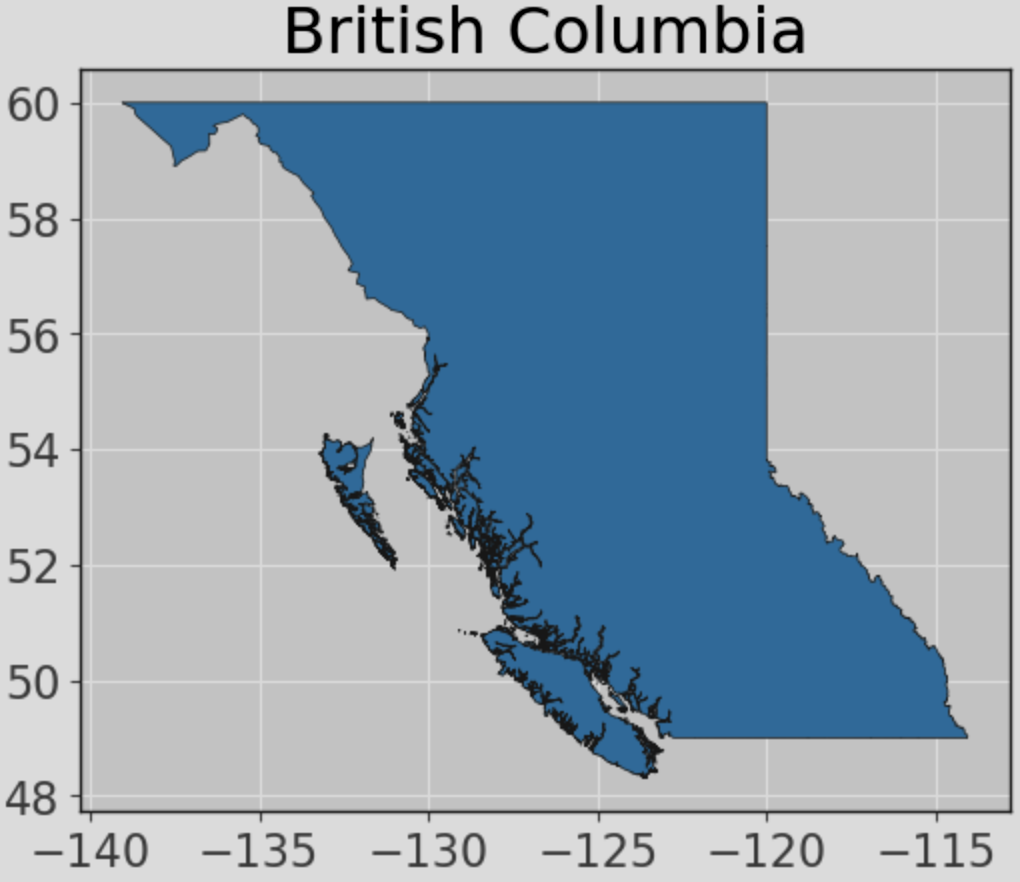
\includegraphics[width=0.5\linewidth, height=3cm]{geopandas.png}

\textbf{Geopandas|}
\smalltext{
It is the primary library for vector data, built on\textbf{shapely} and \textbf{pandas}. It introduces the \textbf{GeoSeries}(storing geometries) and \textbf{GeoDataFrame}(a pandas dataframe with one or more geometry cols). 5 columns of dtype “object” which typically means “strings” in pandas, and we have our one “geometry” column which contains vector data - polygons in this case. MULTIPOLYGONs which just means multiple polygons together - provinces["geometry"][0] 
}

\textbf{Data Acquisition|}
\smalltext{
The \textbf{osmnx} library provides an API to query \textbf{OpenStreetMap (OSM)} for real-world data like road/bike networks, building heights, and city polygons. It can return a networkx graph that can be converted to a GeoDataFrame.
}

\subsection{Geometric Wrangling}
\smalltext{
Spatial wrangling utilizes methods like \textbf{.clip()}(cookie-cutter extraction), \textbf{.buffer()}(adding area around a geometry), and \textbf{.sjoin()}(joining datasets based on spatial location/containment).
}
\begin{lstlisting}[language=python]
# Buffer to create 3m wide paths
joi=gpd.sjoin(polygons, points, how="inner", predicate="contains")
paths["geometry"] = paths.buffer(distance=1.5)
\end{lstlisting}

\subsection{Coordinate Reference Systems}
\smalltext{
A \textbf{CRS} projects the 3D Earth onto a 2D plane. Projections are identified by \textbf{EPSG codes} \textbf{Geographic CRS} e.g.,\textbf{WGS 84 / EPSG:4326} use angular units (degrees) and are best for global positioning. \textbf{Projected CRS} e.g.,\textbf{UTM} or \textbf{Lambert / EPSG:3347} use linear units (meters) and are \textbf{required for calculating lengths and areas} accurately.

No projection is perfect (it’s impossible to perfectly flatten a 3d sphere) and each comprises on minimzing the distortion of shapes, distances, and areas of the Earth. Different CRSs distort spatial data in different ways. So when doing spatial analysis like joining, clipping, mapping, etc. It's important to have all geometries using the same CRS.
}
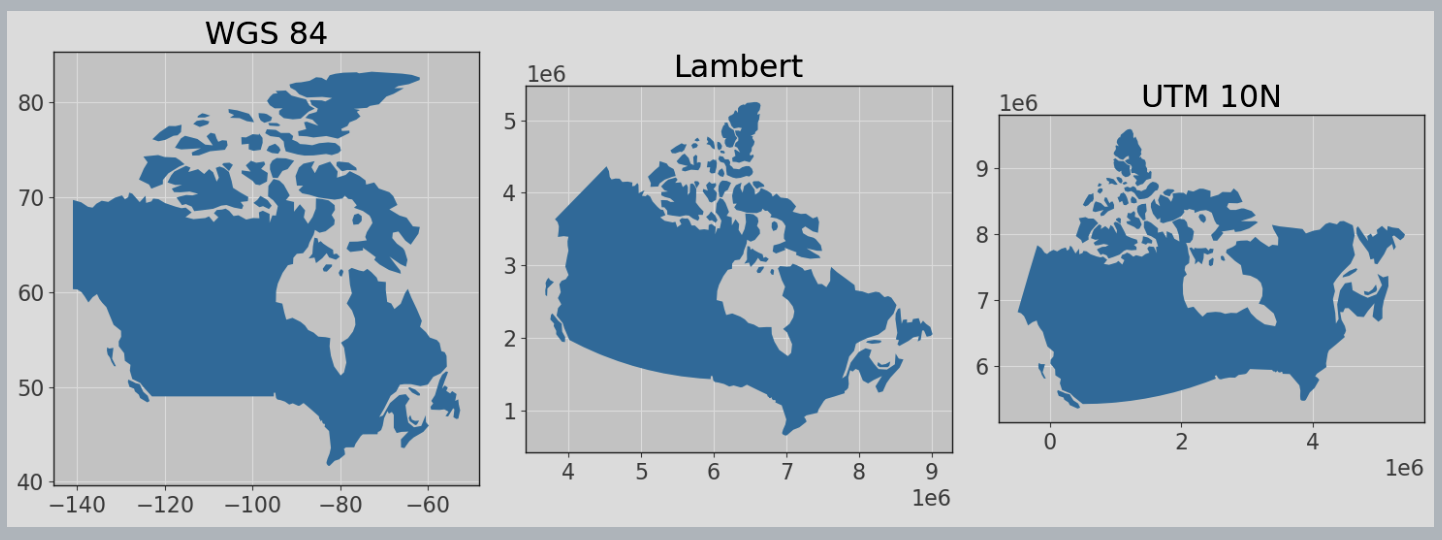
\includegraphics[width=1\linewidth, height=2cm]{projections.png}

% \begin{lstlisting}[language=python]
% gdf = gpd.read_file("data-spatial/provinces")
% # Create GeoDataFrame from Lat/Lon coordinates
% cities_gdf = gpd.GeoDataFrame(df, crs="EPSG:4326", 
%               geometry=gpd.points_from_xy(df["Lon"], df["Lat"]))
% # Fetch polygon boundaries from OpenStreetMap
% vancouver = ox.geocode_to_gdf("Vancouver, Canada")
% # Get bicycle network as a graph and convert to GeoDataFrame
% G = ox.graph_from_place("Stanley Park", network_type="bike")
% bike_gdf = ox.graph_to_gdfs(G, nodes=False).reset_index(drop=True)
% # Clip: Use one layer as a "cookie cutter" for another 
% van_provinces = gpd.clip(gdf, vancouver)
% # Buffer: Add area around a geometry (e.g., 3m wide lane)
% bike_polys = bike_gdf.buffer(distance=1.5)
% # Spatial Join: Merge data based on location (points in polygons)
% joined = gpd.sjoin(van_fsa, van_points, how="inner", redicate="contains")
% # Reproject to linear meters (Lambert EPSG:3347) for accurate calc
% gdf = gdf.to_crs("EPSG:3347")
% gdf["length_m"] = gdf.geometry.length # Length of lines
% gdf["area_m2"] = gdf.area             # Area of polygons
% total_area = gdf.area.sum()
% # Deterministic Interpolation (Nearest Neighbor)
% model = NearestNDInterpolator(x=list(zip(df.x, df.y)), y=df.val)
% # Probabilistic Interpolation (Ordinary Kriging)
% krig = OrdinaryKriging(x=df.x, y=df.y, z=df.val)
% z_grid, sigma = krig.execute("grid", gridx, gridy)
% # Areal Interpolation: Project values from one set of polygons to another
% interp = area_interpolate(source_gdf, target_gdf, intensive_variables=["PM25"])
% gdf.plot(edgecolor="0.2", figsize=(10, 8)) # Quick static plot
% gdf.explore() # Quick interactive map
% # Plotly Interactive Map
% fig = px.choropleth_mapbox(gdf, geojson=gdf.geometry, locations=gdf.index, mapbox_style="open-street-map")
% \end{lstlisting}

\section{Raster Data}
\smalltext{
Raster data is a \textbf{matrix of pixels (cells)} where each cell represents a spatial region containing a specific value. \textbf{Resolution} indicates the ground area per pixel (e.g., 1m vs 8m); "high resolution" implies a smaller pixel size. The core Python package for raster manipulation is \textbf{rasterio}, which handles \textbf{GeoTIFF}(.tif) files containing georeferenced image data. digital image data.
}

\section{Spatial Visualization}
\smalltext{
Geospatial data can be visualized using \code{.plot()} for quick explorations and layer stacking . For interactive zoom and pan functionality, \code{plotly.express} functions like \code{choropleth\_mapbox} are highly effective. \code{Geopandas} also offers \code{.explore()} to create interactive maps. Adding background tiles typically requires converting data to Web Mercator (EPSG:3857) using \code{contextily},.

\code{Kepler.gl} is a powerful web-based tool for spatial visualization with a Python API that supports complex configurations and 3D elements,. It uses a workflow of creating a map instance, adding data, and customizing via a graphical user interface.
}

\section{Spatial Modeling Foundations}
\smalltext{
Spatial modeling is based on Tobler's first fundamental law of geography: "everything is related to everything else, but near things are more related than distant things",. Modeling typically involves \textbf{1.spatial interpolation} to estimate values in unobserved locations \textbf{2.areal interpolation} to project data between different sets of polygons.
}

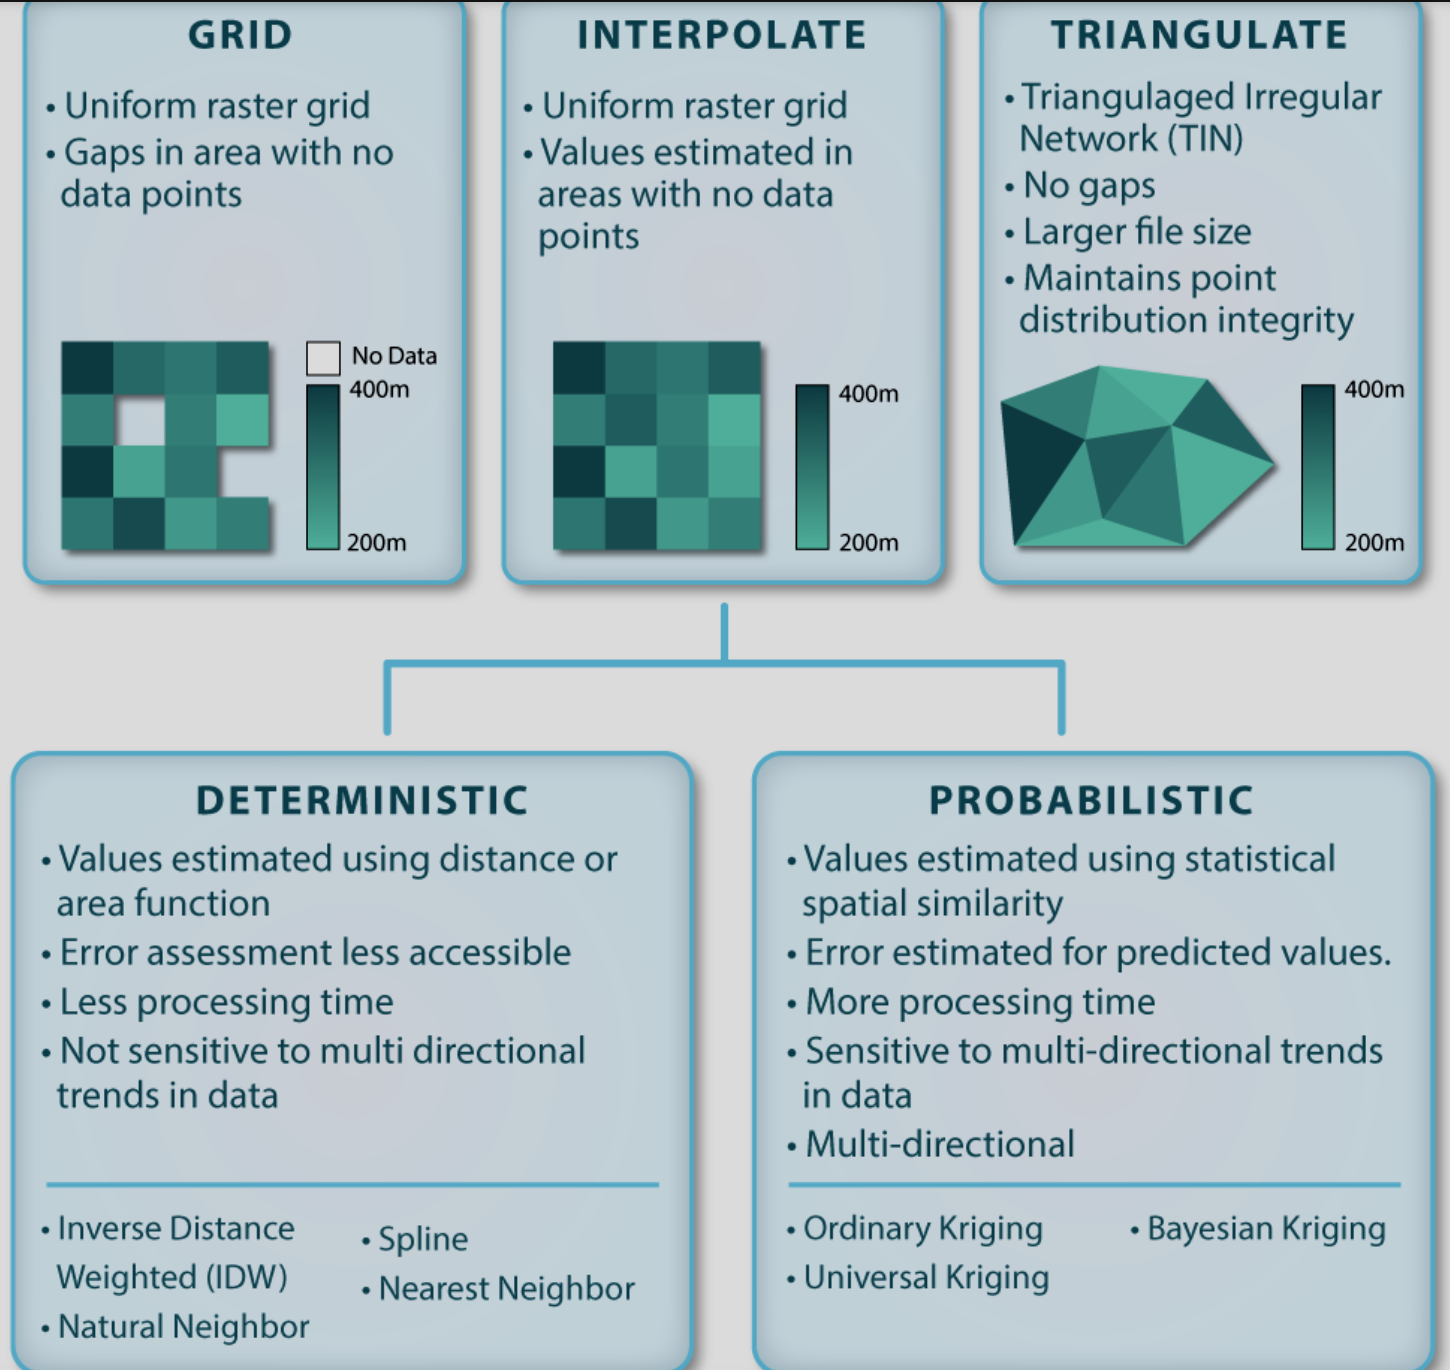
\includegraphics[width=1\linewidth, height=4cm]{spatial-model.png}


\subsection{The Variogram}
\smalltext{
A variogram describes how variance changes with the distance (lag) between locations, serving as the spatial analogue to the time-series ACF,. Key components include the \textbf{range} (the distance where spatial correlation stops), the \textbf{sill} (maximum variance at the range), and the \textbf{nugget} (random or measurement error at zero distance) [20].
}

\subsection{Areal Interpolation}
\smalltext{
Areal interpolation projects values from one set of polygons (source) to another (target), such as mapping pollution data to postal codes. The most common method uses the \code{tobler} library to distribute values based on area proportions,.
}

\subsection{Shortest Path Analysis}
\smalltext{
Network analysis involves finding the optimal path through a network, such as a walking or driving graph. \code{osmnx} is used to load these networks from OpenStreetMap, and Dijkstra's algorithm is the default method for computing the shortest path by length between an origin and destination node,.
}
\begin{lstlisting}[language=python]
route = nx.shortest_path(G, orig_id, dest_id, weight="length")
\end{lstlisting}
    
\end{multicols}
\end{document}
